\chapter{Mechanica van het starre lichaam}\label{ch:b2:rigid-body-mechanics}

Kijk vanaf de stoeprand naar een fietswiel: de spaken vlak bij het wegdek
staan bijna stil en blijven scherp, de spaken bovenaan zijn een veeg die
met twee keer de snelheid van de fietser voorbijtrekt. Elk punt van het
wiel heeft een andere snelheid, en toch is het wiel één voorwerp --- zijn
punten houden hun onderlinge afstanden, en die ene voorwaarde ordent al
hun bewegingen tot twee vectoren, een translatie en een rotatie. Het
volume van jaar 1 behandelde het bijzondere geval van een lichaam dat om
een vaste as draait; dit hoofdstuk geeft de algemene kinematica van een
\omterm{def:b2:rigid-body-mechanics:solid}{star lichaam}, zijn kinetische energie en impulsmoment, de wetten van zijn
beweging, en de wet die elk wiel, elke band, elke rem en elke ladder
beheerst: de wet van Coulomb voor droge wrijving.

\section{Kinematica van een star lichaam}

\begin{definition}[Star lichaam]\label{def:b2:rigid-body-mechanics:solid}
\index{star lichaam}
Een \emph{star lichaam} (of vast lichaam) is een stelsel punten waarvan
de onderlinge afstanden constant blijven: $\|\vect{AB}\|$ hangt niet van
de tijd af voor elk paar $A$, $B$ van zijn punten. Een stelsel waarin elk
punt van het lichaam stilstaat heet een \emph{stelsel verbonden met het
lichaam}.
\end{definition}

\begin{theorem}[Snelheidsveld van een star lichaam]\label{thm:b2:rigid-body-mechanics:field}
\index{rotatievector}\index{snelheidsveld (star lichaam)}
Op elk ogenblik bestaat er een vector $\vect\Omega$, de \emph{\omterm{thm:b2:rigid-body-mechanics:field}{rotatievector}}
van het lichaam (eenheid \unit{rad/s}), zó dat de snelheden van twee
willekeurige punten $A$ en $M$ ervan in een stelsel $\mathcal R$ voldoen aan
\[
\vect v_M = \vect v_A + \vect\Omega\wedge\vect{AM} .
\]
$\vect\Omega$ hangt niet af van de keuze van $A$; een vector $\vect u$ die
vastligt in het lichaam evolueert volgens
$\dd\vect u/\dd t = \vect\Omega\wedge\vect u$.
\end{theorem}

\begin{proof}
Zij $(\vect e_1, \vect e_2, \vect e_3)$ een orthonormale basis verbonden met
het lichaam. Uit $\vect e_i\cdot\vect e_j = \delta_{ij}$ volgt dat de
coëfficiënten $a_{ij} = \dot{\vect e}_i\cdot\vect e_j$ voldoen aan
$a_{ij} + a_{ji} = 0$: de matrix van de afbeelding
$\vect u \mapsto \dot{\vect u}$ (voor
$\vect u$ vast in het lichaam, $\vect u = \sum u_i\vect e_i$ met
constante $u_i$) is antisymmetrisch, en een
antisymmetrische $3\times3$-matrix is de matrix van
$\vect u \mapsto \vect\Omega\wedge\vect u$ met $\Omega_1 = a_{23}$,
$\Omega_2 = a_{31}$,
$\Omega_3 = a_{12}$. Pas haar toe op $\vect u =
\vect{AM}$:
$\vect v_M - \vect v_A = \vect\Omega\wedge\vect{AM}$. Deed $\vect\Omega'$
hetzelfde,
dan was $(\vect\Omega - \vect\Omega')\wedge
\vect{AM} = \vect 0$ voor elke
$M$, dus $\vect\Omega' = \vect\Omega$.
\end{proof}

\begin{remark}[Drie bewegingen]\label{rem:b2:rigid-body-mechanics:motions}
\index{translatie}\index{rotatie om een vaste as}
\emph{Translatie}: $\vect\Omega = \vect 0$, alle punten delen één
snelheid (niet noodzakelijk een rechtlijnige beweging: een cabine van een
reuzenrad transleert langs een cirkel). \emph{\omterm{rem:b2:rigid-body-mechanics:motions}{Rotatie om een vaste as}}
$\Delta$: de punten van $\Delta$ staan stil,
$\vect\Omega = \omega\,\vect e_\Delta$, en een punt op afstand $r$ van de as
beweegt
langs een cirkel met snelheid $r|\omega|$ --- het geval van het volume van
jaar 1. De algemene beweging combineert beide:
$\vect v_M = \vect v_G + \vect\Omega\wedge\vect{GM}$, een translatie met de
snelheid van het
massamiddelpunt plus een rotatie om $G$.
\end{remark}

\begin{definition}[Rollen zonder slippen]\label{def:b2:rigid-body-mechanics:rolling}
\index{rollen zonder slippen}\index{slipsnelheid}
Twee lichamen $S_1$ en $S_2$ raken elkaar in een punt $I$. De
\emph{slipsnelheid} van $S_1$ op $S_2$ is
$\vect v_{\text{glij}} = \vect v_{I \in S_1}
- \vect v_{I \in S_2}$, het
verschil van de snelheden van de twee
materiële punten die op dit ogenblik in $I$ samenvallen. $S_1$
\emph{rolt zonder slippen} op $S_2$ wanneer $\vect v_{\text{glij}} = \vect 0$.
Voor een wiel met straal $R$ dat zonder slippen over een vaste ondergrond
rolt, met middelpuntsnelheid $v_G$ en hoeksnelheid $\omega$, luidt de
voorwaarde $v_G = R\omega$ (met de tekens zó gekozen dat een naar rechts
rollend wiel met de klok mee draait).
\end{definition}

\begin{proof}
Pas \cref{thm:b2:rigid-body-mechanics:field} toe op het wiel tussen $G$ en
het contactpunt $I$:
$\vect v_{I\in S_1} = \vect v_G + \vect\Omega
\wedge\vect{GI}$; met
$\vect v_G = v_G\vect e_x$, $\vect\Omega = -\omega
\vect e_z$ en
$\vect{GI} = -R\vect e_y$ geeft dit $(v_G - R\omega)\vect e_x$,
wat nul moet zijn.
\end{proof}

\begin{example}[Snelheidsveld van een rollend wiel]\label{ex:b2:rigid-body-mechanics:wheel}
Voor het rollende wiel geldt $\vect v_M = \vect\Omega\wedge\vect{IM}$: op
elk ogenblik \emph{draait het wiel om zijn contactpunt}. Het contactpunt
staat stil, het middelpunt beweegt met $v = R\omega$, de top met $2v$, en
een punt van de velg op hoogte $h$ met $\omega\sqrt{2Rh}$, loodrecht op
$\vect{IM}$. Een ventiel beschrijft een cycloïde; een steen die uit het
loopvlak wegschiet, vertrekt met de snelheid van dat velgpunt, tot $2v$
--- daarom zijn de spatlappen van een vrachtwagen geen luxe.
\end{example}

\begin{omfigure}
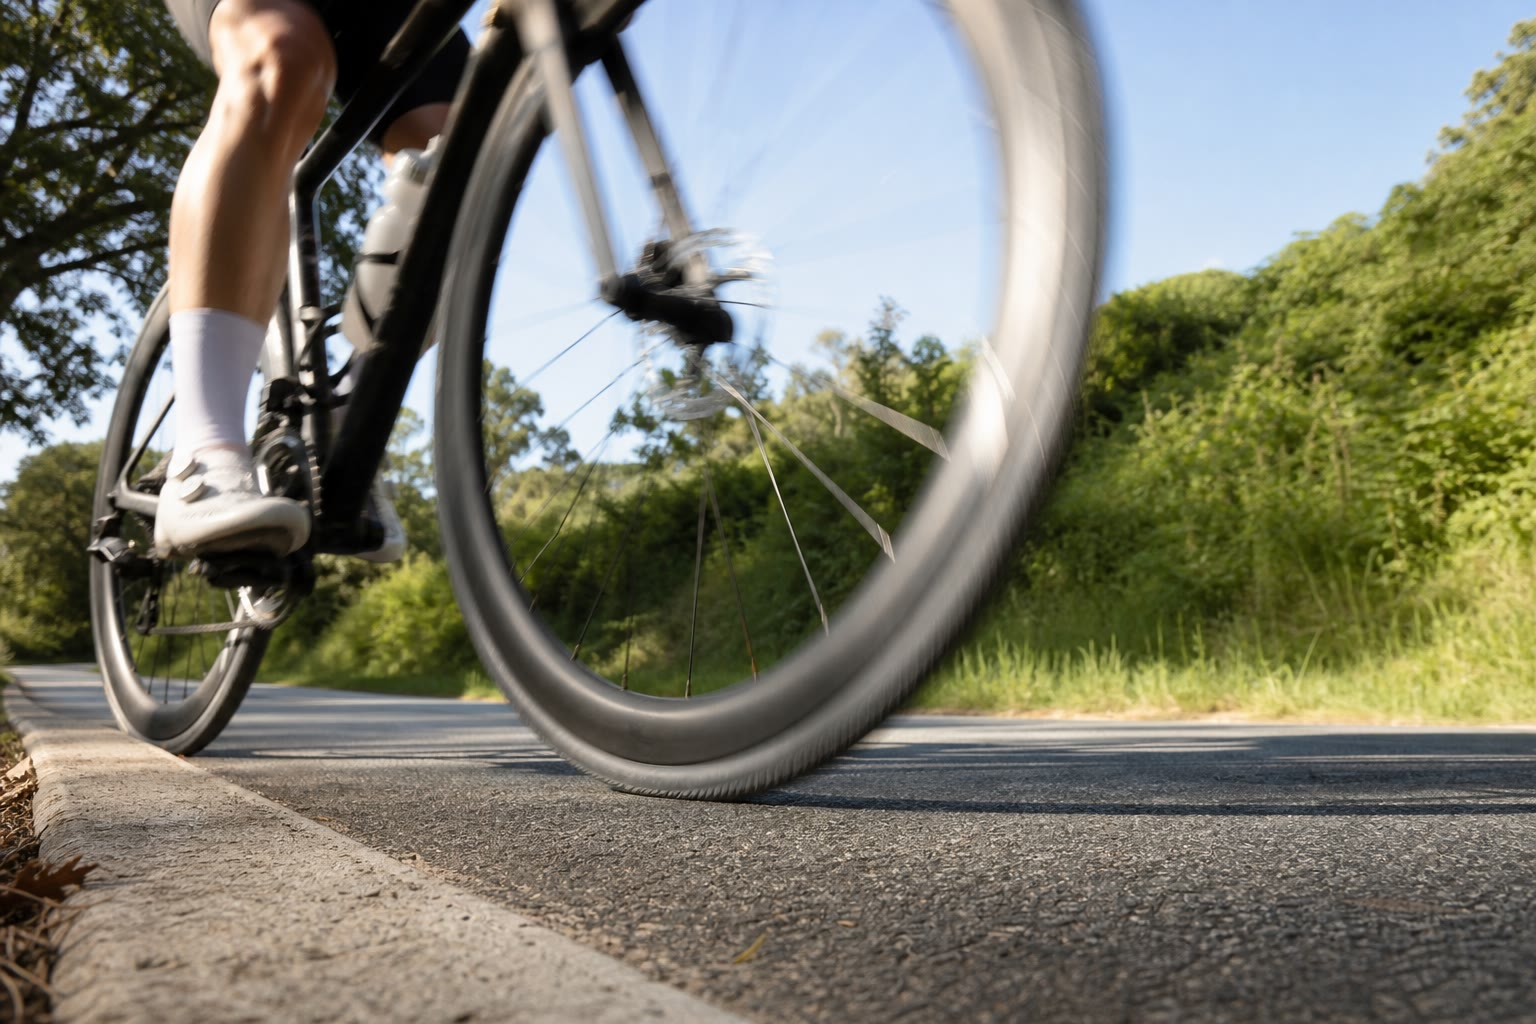
\includegraphics[width=0.58\linewidth]{images/book4/ai/b4-01-bicycle-wheel-blur.jpg}

{\small Een wiel gevangen door een trage sluiter: de spaken vlak bij het
wegdek staan bijna stil en blijven scherp; die bovenaan, die met twee keer
de snelheid van de fiets bewegen, vervagen.}
\end{omfigure}


\begin{omfigure}
\begin{tikzpicture}[font=\small, x=1cm, y=1cm, >=Stealth]
  \begin{scope}
    \draw[thick] (-2.6,0) -- (2.6,0);
    \draw[omDef, thick] (0,1.5) circle (1.5);
    \fill (0,1.5) circle (1.5pt) node[below left, font=\footnotesize] {$G$};
    \fill (0,0) circle (1.5pt) node[below, font=\footnotesize] {$I$};
    \draw[omThm, very thick, ->] (0,1.5) -- (1.2,1.5) node[above, font=\footnotesize] {$\vect v_G$};
    \draw[omThm, very thick, ->] (0,3.0) -- (2.4,3.0) node[pos=0.35, above, font=\footnotesize] {$2\vect v_G$};
    \draw[omThm, very thick, ->] (1.5,1.5) -- (2.7,0.3) node[right, font=\footnotesize] {$\sqrt2\,v_G$};
    \draw[omThm, very thick, ->] (-1.5,1.5) -- (-0.3,2.7) node[above left, font=\footnotesize] {$\sqrt2\,v_G$};
    \draw[omThm, thick, ->] (1.06,0.44) -- (1.41,-0.41);
    \draw[omThm, thick, ->] (-1.06,0.44) -- (-0.71,1.29);
    \node[omThm, font=\footnotesize] at (0.3,0.35) {$\vect v_I = \vect 0$};
    \draw[omProp, ->] (-0.5,2.1) arc[start angle=130, end angle=50, radius=0.75] node[midway, above, font=\footnotesize] {$\omega$};
  \end{scope}
  \begin{scope}[xshift=7.6cm]
    \draw[thick] (-2.6,0) -- (2.6,0);
    \draw[omDef, thick] (0,1.5) circle (1.5);
    \fill (0,0) circle (1.5pt) node[below, font=\footnotesize] {$I$};
    \fill (0,1.5) circle (1.5pt);
    \draw[omThm, ->] (0,1.5) -- ($(0,1.5)!0.45!90:(0,0)$);
    \foreach \a in {30,60,...,330} {
      \coordinate (M) at ({1.5*cos(\a)},{1.5+1.5*sin(\a)});
      \draw[omThm, ->] (M) -- ($(M)!0.45!90:(0,0)$);
    }
    \draw[dashed, omExo] (0,0) -- (1.3,2.25);
    \fill (1.3,2.25) circle (1.2pt) node[right, font=\footnotesize] {$M$};
    \node[font=\footnotesize] at (0,-0.8) {$\vect v_M = \vect\Omega\wedge\vect{IM}$};
    \node[font=\footnotesize, align=center] at (0,3.6) {ogenblikkelijke rotatie\\om het contactpunt};
  \end{scope}
\end{tikzpicture}

{\small Een wiel dat zonder slippen rolt. Links: de snelheden van enkele
punten --- nul in het contactpunt $I$, $v_G = R\omega$ in het middelpunt,
$2v_G$ bovenaan. Rechts: elke snelheid staat loodrecht op het lijnstuk
van het punt naar $I$ en is evenredig met de lengte ervan: op elk
ogenblik draait het wiel om zijn contactpunt.}
\end{omfigure}

\section{Kinetische grootheden van een lichaam}

\begin{proposition}[Impuls, impulsmoment, kinetische energie]\label{prop:b2:rigid-body-mechanics:kinetic}
\index{traagheidsmoment}\index{impulsmoment (lichaam)}\index{kinetische energie (lichaam)}
Voor een lichaam met massa $M$ en massamiddelpunt $G$, in een stelsel $\mathcal R$:
\begin{itemize}
  \item zijn impuls is $\vect p = M\vect v_G$;
  \item draait het om een as $\Delta$ (vast in $\mathcal R$, of door $G$
        gaand en met vaste richting) met hoeksnelheid $\omega$, dan is
        zijn impulsmoment \emph{langs} die as
        $L_\Delta = J_\Delta\,\omega$, waarin
        \[
        J_\Delta = \sum_i m_i r_i^2 = \int r^2\,\dd m
        \]
        zijn \emph{\omterm{prop:b2:rigid-body-mechanics:kinetic}{traagheidsmoment}} om $\Delta$ is ($r$ de afstand tot
        de as; eenheid \unit{kg.m^2});
  \item zijn kinetische energie is (Koenig)
        $E_k = \tfrac12Mv_G^2 +
        E_k^*$, waarin de kinetische energie
        in het zwaartepuntstelsel
        $E_k^* = \tfrac12J_{G}\omega^2$ bedraagt voor een rotatie met
        $\omega$ om een as door $G$ --- en $E_k = \tfrac12J_\Delta\omega^2$
        voor een \omterm{rem:b2:rigid-body-mechanics:motions}{rotatie om een vaste as} $\Delta$.
\end{itemize}
\end{proposition}

\begin{proof}
De stellingen over impuls en die van Koenig werden in het volume van jaar 1
bewezen voor een willekeurig stelsel. Voor de rotatie om $\Delta$ door $O$
heeft een punt op afstand $r_i$ van de as de snelheid $r_i\omega$ langs
een cirkel om de as; zijn impulsmoment om $O$, geprojecteerd op
$\vect e_\Delta$, is $m_ir_i^2\omega$ (de overige componenten, die voor een
symmetrisch lichaam wegvallen, zijn hier niet nodig); sommeer. Kinetische
energie: $\sum\tfrac12m_ir_i^2
\omega^2$.
\end{proof}

\begin{remark}[Wat wordt aangenomen]\label{rem:b2:rigid-body-mechanics:tensor}
Voor een willekeurige rotatie $\vect\Omega$ is de volledige vector
$\vect L_G$ in het algemeen niet evenwijdig met $\vect\Omega$:
$\vect L_G = \mathbf J\,\vect\Omega$ met $\mathbf J$ de
\emph{traagheidstensor}, een
symmetrische matrix waarvan de eigenvectoren de hoofdtraagheidsassen zijn.
Elk lichaam van dit hoofdstuk draait om een vaste as of om een
symmetrieas door $G$, waarvoor $\vect L = J\vect\Omega$ exact geldt; het
algemene geval is voor het volume van jaar 3.
\end{remark}

\begin{proposition}[Traagheidsmomenten]\label{prop:b2:rigid-body-mechanics:inertia}
\index{stelling van Huygens}\index{stelling van de evenwijdige assen}
Voor homogene lichamen met massa $M$, om een as door $G$: dunne staaf met
lengte $\ell$ (as loodrecht), $J = \tfrac1{12}M\ell^2$; dunne ring of
cilinderschil met straal $R$ (eigen as), $J = MR^2$; schijf of volle
cilinder, $J = \tfrac12MR^2$; volle bol, $J = \tfrac25MR^2$; bolschil,
$J = \tfrac23MR^2$. \emph{\omterm{prop:b2:rigid-body-mechanics:inertia}{Stelling van Huygens}} (evenwijdige assen): om
een as $\Delta$ evenwijdig met een as $\Delta_G$ door $G$ op afstand $d$
geldt
\[
J_\Delta = J_{\Delta_G} + Md^2 .
\]
\end{proposition}

\begin{proof}
Voor de staaf: $\int_{-\ell/2}^{\ell/2}x^2\,(M/\ell)\dd x = M\ell^2/12$.
Voor de schijf: ringen met massa $(2M/R^2)r\,\dd r$,
$\int_0^R r^2(2M/R^2)r\,\dd r = MR^2/2$.
Bol: uit symmetrie $J = \tfrac23\int r^2\dd m$ ($r$ de afstand tot het
middelpunt, omdat $x^2 + y^2 = \tfrac23(x^2 + y^2 + z^2)$ gemiddeld over de
drie assen) en $\int r^2\dd m = \int_0^R r^2(3M/R^3)r^2\dd r = \tfrac35MR^2$.
Huygens: met $\vect r_i$ de vector van $\Delta$ naar $m_i$ loodrecht op de
as en $\vect r_i = \vect d + \vect r_i^*$ is
$\sum m_ir_i^2 = Md^2
+ 2\vect d\cdot\sum m_i\vect r_i^* + \sum m_ir_i^{*2}$,
en de middelste som
verdwijnt per definitie van $G$.
\end{proof}

\begin{example}[Een vliegwiel]\label{ex:b2:rigid-body-mechanics:flywheel}
Een stalen schijf van \qty{50}{kg} met straal \qty{30}{cm}:
$J = \tfrac12 \times
50 \times 0.09 = \qty{2.25}{kg.m^2}$; bij
\qty{3000}{rpm} ($\omega =
\qty{314}{rad/s}$) slaat zij
$\tfrac12J\omega^2 = \qty{111}{kJ}$ op, de
kinetische energie van een kleine auto bij \qty{50}{km/h}. Vliegwielen
voor energieopslag laten koolstofvezelrotors op \qty{50000}{rpm} draaien
in vacuüm op magneetlagers: de energie groeit als $\omega^2$, de grens is
de treksterkte van de velg.
\end{example}

\section{Dynamica van een lichaam}

\begin{theorem}[Bewegingswetten van een lichaam]\label{thm:b2:rigid-body-mechanics:laws}
\index{impulsmomentstelling (lichaam)}\index{vermogen van krachten op een lichaam}
In een galileïsch stelsel geldt voor een lichaam waarop uitwendige
krachten $\vect F_i$ in de punten $A_i$ aangrijpen:
\begin{enumerate}
  \item (impuls) $M\,\dd\vect v_G/\dd t = \sum\vect F_i$;
  \item (impulsmoment om $G$, of om een vast punt $O$)
        $\dd\vect L_G/\dd t = \sum\vect{GA_i}\wedge\vect F_i$; geprojecteerd
        op een vaste as $\Delta$, of op een as door $G$ met vaste richting
        waarom het lichaam met $\omega$ draait:
        $J_\Delta\,\dd\omega/\dd t = \mathcal M_\Delta$, de som van de
        momenten van de uitwendige krachten om die as;
  \item (vermogen) het vermogen van een stel krachten op een lichaam is
        $\mathcal P = \vect R\cdot\vect v_A + \vect{\mathcal M}_A\cdot
        \vect\Omega$
        voor elk punt $A$ van het lichaam, met $\vect R$ de
        som van de krachten en $\vect{\mathcal M}_A$ hun totale moment om
        $A$; \emph{de inwendige krachten van een lichaam hebben vermogen
        nul}, en $\dd E_k/\dd t = \mathcal P_{\text{ext}}$.
\end{enumerate}
\end{theorem}

\begin{proof}
(1) en (2) zijn de stellingen van het volume van jaar 1 voor stelsels van
punten (de impulsmomentstelling om $G$ geldt zelfs wanneer $G$ versnelt,
omdat de schijnkrachten van het zwaartepuntstelsel moment nul hebben om
$G$). (3) Met $\vect v_{A_i} = \vect v_A + \vect\Omega
\wedge\vect{AA_i}$:
$\sum\vect F_i\cdot\vect v_{A_i} = \vect R\cdot\vect v_A
+ \sum\vect F_i\cdot(\vect\Omega\wedge\vect{AA_i}) = \vect R\cdot\vect v_A +
\vect\Omega\cdot\sum\vect{AA_i}\wedge\vect F_i$
(gemengd product). Inwendige
krachten: hun som en hun totale moment verdwijnen (actie--reactie, dezelfde
werklijn), vandaar vermogen nul op een lichaam --- \emph{niet} op een
vervormbaar stelsel. De kinetische-energiestelling houdt dan alleen het
uitwendige vermogen over.
\end{proof}

\begin{definition}[Volmaakt scharnier]\label{def:b2:rigid-body-mechanics:pivot}
\index{scharnier (volmaakt)}\index{lager}
Een lichaam draait om een vaste as $\Delta$ in een \emph{volmaakt
scharnier} (een ideaal lager) wanneer de contactkrachten van het lager
moment nul hebben om $\Delta$; zij ontwikkelen dan geen vermogen
($\vect v_A = \vect 0$ op de as, $\mathcal M_\Delta = 0$). Een echt lager
voegt een wrijvingskoppel $-\Gamma_f\operatorname{sgn}\omega$ toe, of een
viskeus koppel $-h\omega$.
\end{definition}

\begin{proposition}[De fysische slinger]\label{prop:b2:rigid-body-mechanics:pendulum}
\index{fysische slinger}\index{samengestelde slinger}
Een lichaam met massa $M$ zwaait om een horizontale vaste as $\Delta$ in
een volmaakt scharnier, met zijn massamiddelpunt op afstand $d$ van de as.
Met $\theta$ de hoek van $\vect{OG}$ met de neerwaartse verticaal geldt
\[
J_\Delta\ddot\theta = -Mgd\sin\theta ,
\]
zodat kleine trillingen de periode $T = 2\pi\sqrt{J_\Delta/Mgd}$ hebben
--- die van een mathematische slinger met lengte $\ell_{\text{eq}} = J_\Delta/Md$.
\end{proposition}

\begin{proof}
Impulsmomentstelling om $\Delta$: het moment van het gewicht is
$-Mgd\sin\theta$, dat van het scharnier nul. Lineariseer.
\end{proof}

\begin{example}[De meterlat]\label{ex:b2:rigid-body-mechanics:rule}
Een meterlat scharnierend aan één uiteinde: $J = \tfrac13M\ell^2$ (Huygens
vanuit $\tfrac1{12}M\ell^2$), $d = \ell/2$,
$\ell_{\text{eq}} = \tfrac23\ell =
\qty{0.667}{m}$ en $T = \qty{1.64}{s}$
--- een slinger van een hele lat
tikt trager dan een puntmassa opgehangen in haar midden (\qty{1.42}{s}) en
sneller dan een in haar uiteinde (\qty{2.0}{s}).
\end{example}

\begin{omfigure}
\begin{tikzpicture}[font=\small, x=1cm, y=1cm, >=Stealth]
  \begin{scope}
    \fill[pattern=north east lines] (-0.6,3.2) rectangle (0.6,3.45); \draw[thick] (-0.6,3.2) -- (0.6,3.2);
    \fill (0,3.1) circle (2pt) node[left, font=\footnotesize] {$O$};
    \draw[dashed] (0,3.1) -- (0,0.2);
    \draw[omDef, very thick, rotate around={25:(0,3.1)}] (-0.12,3.1) rectangle (0.12,0.3);
    \draw[dashed, omExo] (0,3.1) -- ($(0,3.1)+({2.0*sin(25)},{-2.0*cos(25)})$);
    \coordinate (G) at ({0+1.4*sin(25)},{3.1-1.4*cos(25)});
    \fill[omThm] (G) circle (2pt) node[right, font=\footnotesize] {$G$};
    \draw[omThm, very thick, ->] (G) -- ($(G)+(0,-1.0)$) node[below, font=\footnotesize] {$M\vect g$};
    \draw[<->, omExo] (0,1.5) arc[start angle=-90, end angle=-65, radius=1.6] node[midway, below, font=\footnotesize] {$\theta$};
    \node[font=\footnotesize] at (2.1,2.3) {$J_\Delta\ddot\theta = -Mgd\sin\theta$};
    \draw[<->, omExo] (-0.5,3.1) -- ($(-0.5,3.1)+(0,-1.28)$) node[midway, left, font=\footnotesize] {$d$};
  \end{scope}
  \begin{scope}[xshift=7cm]
    \draw[thick] (-2.5,0) -- (2.5,0);
    \draw[omDef, thick] (0,1.2) circle (1.2);
    \fill (0,1.2) circle (1.5pt);
    \draw[omThm, very thick, ->] (0,1.2) -- (0,-0.3) node[right, font=\footnotesize] {$M\vect g$};
    \draw[omProp, very thick, ->] (0,0) -- (0,1.0) node[left, font=\footnotesize, pos=0.7] {$\vect N$};
    \draw[omExo, very thick, ->] (0,0) -- (-1.0,0) node[below, font=\footnotesize] {$\vect T$};
    \draw[very thick, ->] (0.3,2.6) -- (1.5,2.6) node[right, font=\footnotesize] {$\vect F$};
    \draw[omDef, ->] (-0.5,1.7) arc[start angle=130, end angle=50, radius=0.75] node[midway, above, font=\footnotesize] {$\omega$};
    \node[font=\footnotesize, align=left] at (0,-0.9) {rollen zonder slippen: $|T| \le fN$};
  \end{scope}
\end{tikzpicture}

{\small Links: de \omterm{prop:b2:rigid-body-mechanics:pendulum}{fysische slinger} --- het moment van het gewicht om het
scharnier drijft de rotatie aan, de kracht van het scharnier heeft geen
moment. Rechts: de krachten op een wiel dat over een horizontale
ondergrond rolt: gewicht, \omterm{def:b2:rigid-body-mechanics:contact}{normaalkracht} $\vect N$ en tangentiële wrijving
$\vect T$ in het contactpunt, waarvan de grootte begrensd is door de wet
van Coulomb.}
\end{omfigure}

\section{Contactkrachten en wrijving van Coulomb}

\begin{definition}[Contactkracht, normaal en tangentieel]\label{def:b2:rigid-body-mechanics:contact}
\index{normaalkracht}\index{wrijvingskracht}
De kracht die een steunvlak in een contactpunt $I$ op een lichaam
uitoefent, splitst in een \emph{normaalkracht} $\vect N$, loodrecht op het
gemeenschappelijke raakvlak en naar het lichaam toe gericht ($N \ge 0$:
een steunvlak kan alleen duwen), en een \emph{tangentiële component}
$\vect T$ in het raakvlak, de \emph{wrijvingskracht}.
\end{definition}

\begin{theorem}[Wetten van Coulomb voor droge wrijving]\label{thm:b2:rigid-body-mechanics:coulomb}
\index{wrijvingswetten van Coulomb}\index{wrijvingscoëfficiënt}\index{statische wrijving}\index{kinetische wrijving}
Voor twee droge lichamen in contact geldt, met een
\emph{wrijvingscoëfficiënt} $f$ die van de materialen en hun
oppervlaktetoestand afhangt, maar niet van het contactoppervlak en (in
goede benadering) niet van de snelheid:
\begin{itemize}
  \item slippen de lichamen over elkaar
        ($\vect v_{\text{glij}} \ne
        \vect 0$), dan is de
        \omterm{def:b2:rigid-body-mechanics:contact}{wrijvingskracht} tegengesteld aan de
        \omterm{def:b2:rigid-body-mechanics:rolling}{slipsnelheid} en heeft zij de grootte $\|\vect T\| = f\|\vect N\|$
        (\omterm{thm:b2:rigid-body-mechanics:coulomb}{kinetische wrijving});
  \item slippen zij niet, dan is $\|\vect T\| \le f\|\vect N\|$ (\omterm{thm:b2:rigid-body-mechanics:coulomb}{statische
        wrijving}): de \omterm{def:b2:rigid-body-mechanics:contact}{wrijvingskracht} is dan wat de overige
        bewegingswetten vereisen, binnen die grens, en haar richting ligt
        niet op voorhand vast.
\end{itemize}
Een \emph{volmaakt contact} is de idealisatie $f = 0$: $\vect T = \vect 0$.
\end{theorem}
\admitted

\begin{remark}[De wetten van Coulomb lezen]\label{rem:b2:rigid-body-mechanics:reading}
\index{wrijvingskegel}
De eerste wet is een vergelijking, de tweede een ongelijkheid --- en daarin
zit de hele moeilijkheid van wrijvingsvraagstukken. De \emph{werkwijze} is:
\emph{veronderstel} dat er niet geslipt wordt, los $\vect T$ en $\vect N$
op, en \emph{ga na} dat $\|\vect T\| \le f\|\vect N\|$; faalt die toets,
dan slipt het lichaam, is $\|\vect T\| = f\|\vect N\|$ tegengesteld aan de
slip, en wordt het vraagstuk opnieuw opgelost. Meetkundig moet de
contactkracht binnen de \emph{\omterm{rem:b2:rigid-body-mechanics:reading}{wrijvingskegel}} met halve tophoek $\varphi$
blijven, waarbij $\tan\varphi
= f$. Ordegrootten: rubber op droog asfalt
$f \approx 0.8$--$1$, op nat asfalt $0.4$--$0.6$, op ijs $0.1$; staal op
staal $0.15$ droog, $0.05$ gesmeerd; de statische coëfficiënt is in
werkelijkheid iets groter dan de kinetische, en daarom is een slip zo
moeilijk te stoppen als hij eenmaal begonnen is.
\end{remark}

\begin{proposition}[Vermogen van de contactkrachten; rollen zonder slippen]\label{prop:b2:rigid-body-mechanics:power}
\index{rolwrijving}
Het vermogen van de contactkrachten op een lichaam dat over een vast
steunvlak beweegt, is $\mathcal P = \vect T\cdot\vect v_{I\in S}$ (de
\omterm{def:b2:rigid-body-mechanics:contact}{normaalkracht} staat loodrecht op de snelheid van het contactpunt, die in
het raakvlak ligt). Bij \emph{\omterm{def:b2:rigid-body-mechanics:rolling}{rollen zonder slippen}} is dat vermogen nul:
wrijving verricht dan geen arbeid, al kan zij onmisbaar zijn voor de
beweging. Bij glijden is het $-f N v_{\text{glij}} < 0$: warmte.
\end{proposition}

\begin{proof}
$\mathcal P = (\vect N + \vect T)\cdot\vect v_{I\in S}$ en
$\vect
v_{I\in S} = \vect v_{\text{glij}}$ ligt in het raakvlak, zodat
alleen
$\vect T$ bijdraagt; die bijdrage is nul wanneer de \omterm{def:b2:rigid-body-mechanics:rolling}{slipsnelheid} nul is,
en $-fNv_{\text{glij}}$ wanneer de lichamen slippen ($\vect T$
tegengesteld aan $\vect
v_{\text{glij}}$). Echt rollen dissipeert een
beetje door de vervorming van band en ondergrond (\emph{\omterm{prop:b2:rigid-body-mechanics:power}{rolwrijving}},
gemodelleerd door een klein koppel $\Gamma_r = \mu_rNR$ of een equivalente
kracht $\mu_rN$, met $\mu_r \approx 0.01$ voor een band op een weg): een
ander en veel kleiner effect.
\end{proof}

\begin{method}[Een lichaam dat een helling af rolt]\label{met:b2:rigid-body-mechanics:incline}
\index{een helling af rollen}
Een homogeen lichaam met straal $R$, massa $M$ en \omterm{prop:b2:rigid-body-mechanics:kinetic}{traagheidsmoment}
$J =
kMR^2$ om zijn as ($k = 1$ ring, $\tfrac12$ schijf, $\tfrac25$ bol)
wordt
losgelaten op een helling met hoek $\alpha$ en wrijvingscoëfficiënt $f$.
Neem aan dat het zonder slippen rolt:
\begin{enumerate}
  \item impuls langs de helling: $M\dot v = Mg\sin\alpha - T$; normaal:
        $N = Mg\cos\alpha$;
  \item impulsmoment om $G$: $kMR^2\dot\omega = TR$;
  \item geen slip: $v = R\omega$, vandaar $T = kM\dot v$ en
        \[
        \dot v = \frac{g\sin\alpha}{1 + k} , \qquad T = \frac{k}{1 + k}\,
        Mg\sin\alpha ;
        \]
  \item toets: $T \le fN \iff \tan\alpha \le f\,\dfrac{1 + k}{k}$.
        Boven die helling slipt het lichaam, $T = fMg\cos\alpha$,
        $\dot v =
        g(\sin\alpha - f\cos\alpha)$ en
        $\dot\omega = fg\cos\alpha/kR$.
\end{enumerate}
Energietoets (geen slip, wrijving zonder vermogen):
$\tfrac12(1 + k)Mv^2 =
Mgh$ geeft $v = \sqrt{2gh/(1 + k)}$ --- een bol wint
van een schijf, die
wint van een ring, onafhankelijk van massa en straal.
\end{method}

\begin{omfigure}
\begin{tikzpicture}[font=\small, x=1cm, y=1cm, >=Stealth]
  \begin{scope}
    \draw[thick] (0,0) -- (5.5,0) -- (0,2.6) -- cycle;
    \draw (0.9,0) arc[start angle=180, end angle=155, radius=0.9] node[left, font=\footnotesize, xshift=-2pt] {};
    \node[font=\footnotesize] at (4.6,0.25) {$\alpha$};
    \draw (5.5,0) -- (4.7,0) arc[start angle=180, end angle=155, radius=0.8];
    \coordinate (I) at (2.2,1.56);
    \coordinate (G) at ($(I)+(155:-0.0)+(65:0.8)$);
    \draw[omDef, thick] (G) circle (0.8);
    \fill (G) circle (1.5pt);
    \draw[omThm, very thick, ->] (G) -- ($(G)+(0,-1.3)$) node[below, font=\footnotesize] {$M\vect g$};
    \draw[omProp, very thick, ->] (I) -- ($(I)+(65:1.0)$) node[above left, font=\footnotesize, pos=0.9] {$\vect N$};
    \draw[omExo, very thick, ->] (I) -- ($(I)+(155:0.9)$) node[above, font=\footnotesize] {$\vect T$};
    \draw[->, thick] ($(G)+(65:1.1)$) -- ($(G)+(65:1.1)+(-25:1.2)$) node[right, font=\footnotesize] {$\vect v$};
    \node[font=\footnotesize, align=left] at (4.6,1.7) {$\dot v = \dfrac{g\sin\alpha}{1+k}$};
  \end{scope}
  \begin{scope}[xshift=7.6cm]
    \begin{axis}[omaxis, axis x line=bottom, axis y line=left, width=5.6cm, height=4.2cm,
        xlabel={$\alpha$ (graden)}, ylabel={$\dot v/g$}, xmin=0, xmax=90, ymin=0, ymax=1.05,
        xlabel style={at={(axis description cs:0.5,-0.12)}, anchor=north},
        ylabel style={at={(axis description cs:-0.2,0.5)}, rotate=90, anchor=south},
        xtick={0,30,60,90}, ytick={0,0.5,1}, samples=200, legend style={font=\scriptsize, at={(0.03,0.97)}, anchor=north west, draw=none, fill=none}]
      \addplot[omThm, thick, domain=0:56.3] {sin(x)/1.5};
      \addplot[omThm, thick, domain=56.3:90] {sin(x)-0.5*cos(x)};
      \addplot[omDef, thick, dashed, domain=0:90] {sin(x)};
      \legend{schijf, , zonder wrijving}
      \draw[dotted] (axis cs:56.3,0) -- (axis cs:56.3,0.83);
      \node[font=\scriptsize, anchor=west] at (axis cs:57,0.3) {slipt};
    \end{axis}
  \end{scope}
\end{tikzpicture}

{\small Links: de krachten op een lichaam dat een helling af rolt ---
gewicht in $G$, \omterm{def:b2:rigid-body-mechanics:contact}{normaalkracht} en wrijving in het contactpunt. Rechts: de
versnelling van een schijf ($k = \tfrac12$) als functie van de helling
voor $f = 0.5$: zij rolt zonder slippen zolang $\tan\alpha \le 3f$, slipt
daarna, en haar versnelling volgt $g(\sin\alpha - f\cos\alpha)$, steeds
onder de wrijvingsloze $g\sin\alpha$.}
\end{omfigure}

\begin{example}[Waarom een auto wrijving nodig heeft om te versnellen]\label{ex:b2:rigid-body-mechanics:car}
Een auto met voorwielaandrijving: de motor oefent een koppel uit op de
voorwielen; de enige uitwendige horizontale kracht op de auto is de
wrijving van de weg op de banden, en het is die kracht die de auto
versnelt. Rust het hele gewicht op de aangedreven wielen, dan is de
maximale versnelling $fg \approx \qty{8}{m/s^2}$ op droog asfalt --- en de
helft daarvan als slechts de helft van het gewicht op de aangedreven as
rust; op ijs $\qty{1}{m/s^2}$. De arbeid van de motor wordt niet door de weg
verricht (het contactpunt staat immers stil): het is inwendige arbeid, die
de transmissie in kinetische energie omzet --- net zoals de inwendige
krachten van de spieren van een wandelaar, en niet de grond, zijn energie
leveren.
\end{example}

\begin{example}[De overgang van glijden naar rollen]\label{ex:b2:rigid-body-mechanics:bowling}
Een bowlingbal wordt glijdend losgelaten met $v_0$ en zonder rotatie.
\omterm{thm:b2:rigid-body-mechanics:coulomb}{Kinetische wrijving} $fMg$ remt het middelpunt af ($\dot v = -fg$) en brengt
de bal op toeren ($\tfrac25MR^2\dot\omega = fMgR$, $\dot\omega = 5fg/2R$)
tot $v = R\omega$: op $t_1 = 2v_0/7fg$, met $v_1 = \tfrac57v_0$. Vanaf dan
rolt hij zonder slippen met constante snelheid. Twee zevende van de
snelheid, en $1 - (\tfrac57)^2\tfrac75 = \tfrac27$ van de kinetische
energie, gaan in de glijfase als warmte verloren --- wat $f$ ook is; $f$
bepaalt alleen hoe snel.
\end{example}

\begin{omfigure}
\begin{tikzpicture}
\begin{axis}[omaxis, axis x line=bottom, axis y line=left, width=7.6cm, height=4.4cm,
    xlabel={$t/t_1$}, ylabel={}, xmin=0, xmax=2, ymin=0, ymax=1.15,
    xlabel style={at={(axis description cs:0.5,-0.12)}, anchor=north},
    xtick={0,1,2}, ytick={0.714,1}, yticklabels={$\tfrac57v_0$, $v_0$}, samples=100,
    legend style={font=\scriptsize, at={(0.97,0.35)}, anchor=east, draw=none, fill=none}]
  \addplot[omThm, thick, domain=0:1] {1-0.2857*x};
  \addplot[omThm, thick, domain=1:2] {0.714};
  \addplot[omDef, thick, domain=0:1] {0.714*x};
  \addplot[omDef, thick, domain=1:2] {0.714};
  \legend{$v_G$, , $R\omega$}
  \draw[dotted] (axis cs:1,0) -- (axis cs:1,0.714);
\end{axis}
\end{tikzpicture}

{\small Een bal die glijdend en zonder rotatie wordt losgelaten:
\omterm{thm:b2:rigid-body-mechanics:coulomb}{kinetische wrijving} remt het middelpunt en brengt de bal op toeren,
lineair in de tijd, tot $R\omega$ de waarde $v_G$ inhaalt bij
$\tfrac57v_0$; vanaf dan rolt de bal zonder slippen en houdt de wrijving
op te werken.}
\end{omfigure}

\section{Oefeningen}

\begin{exercise}[$\star$]\label{exo:b2:rigid-body-mechanics:1}
\omterm{prop:b2:rigid-body-mechanics:kinetic}{Traagheidsmomenten}: (a) een staaf van \qty{1.0}{m} en \qty{0.50}{kg} om een
loodrechte as door haar midden, en vervolgens door een uiteinde; (b) een
schijf van \qty{2.0}{kg} met straal \qty{20}{cm} om haar as, en vervolgens
om een evenwijdige as door haar rand; (c) een biljartbal van \qty{0.16}{kg}
met diameter \qty{57}{mm}. (d) Een dunne ring en een volle schijf met
dezelfde massa en straal: welke verzet zich meer tegen het op gang
brengen, en met welke factor?
\end{exercise}

\begin{exercise}[$\star$]\label{exo:b2:rigid-body-mechanics:2}
Een fiets rijdt \qty{18}{km/h} op wielen met diameter \qty{70}{cm}.
Hoeksnelheid van de wielen; snelheid, in het stelsel van de weg, van het
ventiel wanneer het bovenaan, onderaan en vooraan het wiel staat (ter
hoogte van de as); snelheid van het loopvlak ten opzichte van het frame
van de fiets. Een steen die in het loopvlak vastzit, komt bovenaan los:
met welke snelheid vertrekt hij?
\end{exercise}

\begin{exercise}[$\star$]\label{exo:b2:rigid-body-mechanics:3}
Een vliegwiel is een stalen schijf van \qty{40}{kg} met straal \qty{25}{cm}.
(a) Opgeslagen energie bij \qty{6000}{rpm}. (b) Constant koppel nodig om
het vanuit rust in \qty{2.0}{min} op toeren te brengen; vermogen aan het
eind daarvan. (c) In een bus moet het \qty{20}{kW} leveren gedurende
\qty{10}{s}: tot welk toerental zakt het? (d) Waarom draaien snelle
vliegwielen in vacuüm?
\end{exercise}

\begin{exercise}[$\star$]\label{exo:b2:rigid-body-mechanics:4}
Een homogene schijf met straal $R$ zwaait in een verticaal vlak om een
horizontale as door een punt van haar rand. \omterm{prop:b2:rigid-body-mechanics:kinetic}{Traagheidsmoment} om die as;
periode van kleine trillingen voor $R = \qty{20}{cm}$; lengte van de
equivalente mathematische slinger. Dezelfde vragen voor de as op afstand
$R/2$ van het middelpunt. Waar moet de as liggen voor de kortste periode?
\end{exercise}

\begin{exercise}[$\star\star$]\label{exo:b2:rigid-body-mechanics:5}
Een ring, een schijf en een bol met dezelfde straal worden samen
losgelaten aan de top van een helling van \qty{2.0}{m} hoog met
hellingshoek \qty{20}{\degree}, $f =
0.30$. (a) Ga na dat alle drie zonder
slippen rollen. (b) Snelheid onderaan voor elk; volgorde van aankomst.
(c) Benodigde tijd voor elk. (d) Toon aan dat de \omterm{def:b2:rigid-body-mechanics:contact}{wrijvingskracht} op de bol
$\tfrac27Mg\sin\alpha$ is en dat zij geen arbeid verricht. (e) Bij welke
helling begint de ring te slippen? En de bol?
\end{exercise}

\begin{exercise}[$\star\star$]\label{exo:b2:rigid-body-mechanics:6}
\emph{Schijfrem.} Een wiel met zijn remschijf heeft $J = \qty{1.2}{kg.m^2}$
en draait op \qty{900}{rpm}; twee remblokken drukken op de schijf op een
gemiddelde straal van \qty{12}{cm}, elk met een \omterm{def:b2:rigid-body-mechanics:contact}{normaalkracht} van
\qty{800}{N}, $f = 0.40$. Remkoppel; hoekvertraging; tijd en aantal
omwentelingen tot stilstand; vrijgekomen warmte, en temperatuurstijging
van de stalen schijf van \qty{1.5}{kg} ($c = \qty{470}{J/(kg.K)}$) als zij
alles opneemt.
\end{exercise}

\begin{exercise}[$\star\star$]\label{exo:b2:rigid-body-mechanics:7}
\emph{Machine van Atwood met een echte katrol.} Massa's $m_1 = \qty{2.0}{kg}$
en $m_2 = \qty{1.5}{kg}$ hangen aan een touw over een katrol met straal
$R =
\qty{10}{cm}$ en \omterm{prop:b2:rigid-body-mechanics:kinetic}{traagheidsmoment} $J = \qty{5.0e-3}{kg.m^2}$ in een
volmaakt
scharnier; het touw slipt niet op de katrol. (a) Waarom zijn de twee
touwspanningen verschillend? (b) Vergelijkingen voor de twee massa's en de
katrol; versnelling. (c) De twee spankrachten. (d) Vergelijk met de
massaloze katrol; vind de versnelling terug langs de energie.
\end{exercise}

\begin{exercise}[$\star\star$]\label{exo:b2:rigid-body-mechanics:8}
\emph{De ladder.} Een homogene ladder met lengte $\ell$ en massa $m$ leunt
onder een hoek $\theta$ met de horizontaal tegen een gladde verticale muur;
de grond heeft wrijvingscoëfficiënt $f$. (a) Krachten en hun momenten om
de voet; evenwichtsvergelijkingen. (b) Toon aan dat evenwicht
$\tan\theta \ge 1/2f$ vereist. (c) Minimale hoek voor $f = 0.40$. (d) Iemand
met massa $3m$ klimt op de ladder die onder \qty{60}{\degree} staat: hoe hoog
(als fractie van $\ell$) kan die persoon komen?
\end{exercise}

\begin{exercise}[$\star\star$]\label{exo:b2:rigid-body-mechanics:9}
\emph{Terugspin.} Een biljartbal wordt zó gestoten dat hij vertrekt met
middelpuntsnelheid $v_0$ en terugspin $\omega_0$ (rotatie tegengesteld aan
rollen). Wrijvingscoëfficiënt $f$. (a) Vergelijkingen voor $v$ en $\omega$
tijdens het glijden. (b) Tijdstip waarop hij zonder slippen begint te
rollen en zijn snelheid dan, als functie van $v_0$ en $R\omega_0$.
(c) Voorwaarde op $R\omega_0$ opdat de bal naar de speler terugkeert.
(d) Getallen: $v_0 = \qty{2.0}{m/s}$, $R\omega_0 = \qty{6.0}{m/s}$, $f = 0.2$,
$R = \qty{2.9}{cm}$.
\end{exercise}

\begin{exercise}[$\star\star\star$]\label{exo:b2:rigid-body-mechanics:10}
\emph{De klos.} Een klos (massa $M$, \omterm{prop:b2:rigid-body-mechanics:kinetic}{traagheidsmoment} $J = kMR^2$ om zijn
as, buitenstraal $R$) ligt op een horizontale tafel; aan een draad die om
zijn binnenste naaf met straal $r < R$ gewikkeld is, wordt horizontaal
getrokken met een kracht $F$, waarbij de draad aan de \emph{onderkant} van
de naaf afloopt. (a) Schrijf, aannemend dat de klos zonder slippen rolt, de
vergelijkingen voor impuls en impulsmoment op en bepaal de versnelling van
het middelpunt; welke kant rolt de klos op? (b) Vereiste \omterm{def:b2:rigid-body-mechanics:contact}{wrijvingskracht},
en de voorwaarde op $F$ om niet te slippen. (c) Dezelfde vragen als er
onder een hoek $\beta$ boven de horizontaal getrokken wordt; toon aan dat
de klos stilblijft wanneer $\cos\beta = r/R$, en verklaar dat meetkundig
(ogenblikkelijke as door het contactpunt). (d) Wat gebeurt er voor
$\cos\beta < r/R$?
\end{exercise}

\begin{exercise}[$\star\star\star$]\label{exo:b2:rigid-body-mechanics:11}
\emph{Waar men een biljartbal moet raken.} Een keu geeft een horizontale
stoot $P$ (zeer korte kracht) aan een bal met straal $R$ in rust, op hoogte
$h$ boven het laken. (a) Impuls en impulsmoment vlak na de stoot (wrijving
verwaarloosbaar tijdens de stoot). (b) Toon aan dat de bal meteen zonder
slippen rolt als $h = \tfrac75R$, met voorwaartse rotatie erboven en
terugspin eronder. (c) Voor $h = R$ (raak in het midden): hoe ver glijdt de
bal voordat hij rolt, met $f = 0.2$ en $v_0 = \qty{3}{m/s}$? (d) Waarom
ligt de band van een biljart op hoogte $\tfrac75R$?
\end{exercise}

\begin{exercise}[$\star\star\star$]\label{exo:b2:rigid-body-mechanics:12}
\emph{Cilinder in een schaal.} Een volle cilinder met straal $r$ rolt
zonder slippen binnen een vast cilindrisch oppervlak met straal $R > r$,
de assen horizontaal en evenwijdig. Zij $\theta$ de hoek van de
verbindingslijn van de middelpunten met de verticaal. (a) Druk de
hoeksnelheid van de cilinder om zijn eigen as uit in $\dot\theta$ (tip:
het contactpunt staat stil). (b) Kinetische en potentiële energie; toon
aan dat de periode van kleine trillingen $T = 2\pi\sqrt{3(R - r)/2g}$ is.
(c) Vergelijk met een punt dat wrijvingsloos in de schaal glijdt.
(d) Minimale wrijvingscoëfficiënt om zonder slippen te rollen bij
amplitude $\theta_0$ (kleine hoeken).
\end{exercise}

\section{Vraagstuk: Een voertuig op wielen}

\begin{problem}[{Weekendvraagstuk --- wat een auto van zijn banden vraagt:
rollen, versnellen, remmen, en de ene kracht die het allemaal doet}]
\label{pb:b2:rigid-body-mechanics:1}

Een auto met massa $M = \qty{1200}{kg}$ heeft een wielbasis $L = \qty{2.6}{m}$;
zijn massamiddelpunt ligt op hoogte $h = \qty{0.55}{m}$ en op horizontale
afstanden $a = \qty{1.1}{m}$ van de vooras en $b = \qty{1.5}{m}$ van de
achteras. Elk van de vier wielen heeft straal $R = \qty{0.31}{m}$, massa
$m =
\qty{15}{kg}$ en \omterm{prop:b2:rigid-body-mechanics:kinetic}{traagheidsmoment} $J = \qty{1.0}{kg.m^2}$ om zijn as.
Wrijvingscoëfficiënt band--weg $f = 0.80$ (droog); rolwrijvingscoëfficiënt
$\mu_r = 0.012$. $g = \qty{9.81}{m/s^2}$.

\medskip
\noindent\textbf{Deel I --- Rollen.}
\begin{enumerate}
  \item De auto rijdt $v = \qty{90}{km/h}$. Hoeksnelheid van de wielen;
        snelheid, in het stelsel van de weg, van het bovenste, het
        onderste en het voorste punt van een band.
  \item Totale kinetische energie van de auto, met de translatie van het
        geheel en de rotatie van de vier wielen apart; welke fractie
        vertegenwoordigen de rotaties van de wielen?
  \item In rust op een vlakke weg: de \omterm{def:b2:rigid-body-mechanics:contact}{normaalkrachten} $N_f$ (beide
        voorwielen samen) en $N_r$ (beide achterwielen) uit de
        vergelijkingen voor impuls en impulsmoment --- welke as draagt
        meer?
  \item Het rolwrijvingskoppel op elk wiel is $\mu_rNR$. Vermogen
        gedissipeerd door \omterm{prop:b2:rigid-body-mechanics:power}{rolwrijving} bij \qty{90}{km/h}; vergelijk met de
        luchtweerstand $\tfrac12\rho C_xSv^2$ met
        $C_xS =
        \qty{0.70}{m^2}$, $\rho = \qty{1.2}{kg/m^3}$.
  \item De motor wordt afgezet en de auto rolt uit op een vlakke weg:
        schrijf de vergelijking voor $v(t)$ op (neem de traagheid van de
        wielen mee als een effectieve massa) en schat de afstand om van
        \qty{90}{km/h} tot \qty{45}{km/h} te vertragen, eerst zonder
        luchtweerstand, daarna met alleen luchtweerstand.
\end{enumerate}

\medskip
\noindent\textbf{Deel II --- Versnellen.}
De auto heeft voorwielaandrijving; de motor oefent een koppel $\Gamma$ uit
op de twee voorwielen samen. Verwaarloos hier luchtweerstand en \omterm{prop:b2:rigid-body-mechanics:power}{rolwrijving}.
\begin{enumerate}[resume]
  \item Teken de uitwendige krachten op de hele auto. Welke kracht
        versnelt hem? Wat is het vermogen van de weg op de auto, en waar
        komt de kinetische energie vandaan?
  \item Schrijf de impulsvergelijking van de auto op, de
        impulsmomentvergelijking van de voorwielen om hun as, en de
        slipvrije voorwaarde; toon aan dat de versnelling
        $\dot v =
        \Gamma/R\,/\,(M + 4J/R^2)$ is en bereken de effectieve
        massa.
  \item Impulsmoment om het massamiddelpunt voor de hele auto (beschouw de
        impulsmomenten van de wielen als verwaarloosbaar): toon aan dat de
        gewichtsverplaatsing bij versnelling $\dot v$ gelijk is aan
        $N_r - N_r^0 =
        Mh\dot v/L$ --- de vooras wordt ontlast, de
        achteras belast.
  \item Maximale versnelling zonder dat de aangedreven (voor)wielen
        doorslippen: toon aan dat $\dot v_{\max} = fgb/(L + fh)$ en bereken
        die; hetzelfde voor een auto met achterwielaandrijving,
        $\dot v_{\max} =
        fga/(L - fh)$. Welke opzet versnelt harder, en
        waarom leggen dragsters het gewicht achterin?
  \item Motorkoppel aan de wielen nodig voor $\dot v_{\max}$; het
        bijbehorende vermogen bij \qty{50}{km/h}.
  \item Dezelfde auto op ijs ($f = 0.10$): maximale versnelling en de tijd
        om \qty{50}{km/h} te bereiken.
  \item Wat doet de \omterm{def:b2:rigid-body-mechanics:contact}{wrijvingskracht} op de voorbanden met de band ---
        glijden of niet --- en waarom versnelt een doorslippend wiel op ijs
        de auto \emph{minder} dan een grijpend wiel?
\end{enumerate}

\medskip
\noindent\textbf{Deel III --- Remmen.}
\begin{enumerate}[resume]
  \item De remmen leggen een koppel op elk wiel. Toon aan dat voor een
        wiel dat blijft rollen de remkracht op de auto de wrijving van de
        weg op de band is, en dat het remkoppel per wiel door $fN_iR$
        begrensd wordt.
  \item Gewichtsverplaatsing bij vertraging $\gamma$: belasting van de
        vooras $N_f = Mg\,b/L + Mh\gamma/L$; getallen bij $\gamma = fg$.
  \item Maximale vertraging met alle vier de wielen op de grens van
        slippen; remweg vanaf \qty{90}{km/h} op droge weg, en op natte weg
        ($f = 0.45$).
  \item Zijn de remmen zó afgesteld dat de koppels voor en achter gelijk
        zijn, welke as blokkeert dan het eerst bij hard remmen? Waarom is
        een geblokkeerde achteras gevaarlijk (denk aan de richting van de
        \omterm{def:b2:rigid-body-mechanics:contact}{wrijvingskracht} op een glijdende band)?
  \item Een wiel blokkeert en glijdt: vertraging vanaf de weg, en welke
        fractie van het maximale remvermogen verloren gaat met
        $f_{\text{kinetisch}} =
        0.7$ tegenover $f_{\text{statisch}} = 0.8$.
        Leg uit wat een antiblokkeersysteem doet en waarom het de remmen
        laat pulseren.
  \item In de remmen vrijgekomen warmte vanaf \qty{90}{km/h};
        temperatuurstijging van vier stalen schijven van \qty{6}{kg}
        ($c = \qty{470}{J/(kg.K)}$); waarom hebben bergwegen
        uitwijkstroken voor vrachtwagens?
  \item Een elektrische auto wint remenergie terug via zijn motor met een
        rendement van \qty{70}{\%}: teruggewonnen energie per stop vanaf
        \qty{90}{km/h}; aantal van zulke stops dat een accu van
        \qty{50}{kWh} waard is.
\end{enumerate}

\medskip
\noindent\textbf{Deel IV --- Bochten nemen en een wiel van de grond.}
\begin{enumerate}[resume]
  \item De auto rijdt op een vlakke weg een cirkel met straal
        $\rho = \qty{50}{m}$ met snelheid $v$: de \omterm{def:b2:rigid-body-mechanics:contact}{wrijvingskrachten} moeten
        $Mv^2/\rho$ leveren. Maximale bochtsnelheid op droge en op natte
        weg.
  \item Impulsmoment om het massamiddelpunt langs de bewegingsrichting:
        toon aan dat de buitenste wielen extra belast worden met
        $\Delta N =
        Mv^2h/\rho w$, waarin $w = \qty{1.5}{m}$ de
        spoorbreedte is; snelheid waarbij de binnenste wielen loskomen
        ($\Delta N = Mg/2$), en vergelijk met de \omterm{def:b2:rigid-body-mechanics:rolling}{slipsnelheid}: kantelt deze
        auto eerder of slipt hij eerder?
  \item De bocht heeft een verkanting onder een hoek $\beta$. Toon aan dat
        bij de snelheid $v = \sqrt{g\rho\tan\beta}$ helemaal geen wrijving
        nodig is; waarde voor $\beta = \qty{10}{\degree}$.
  \item Een wiel wordt vrij gekrikt en met de hand op \qty{60}{rpm}
        gebracht; zijn \omterm{def:b2:rigid-body-mechanics:pivot}{lager} oefent een wrijvingskoppel van \qty{0.05}{N.m}
        uit. Hoe lang blijft het draaien? Verloren kinetische energie.
  \item Het draaiende wiel wordt op de weg neergelaten (auto in rust, wiel
        op \qty{60}{rpm}, $N = \qty{3}{kN}$): glijtijd voordat het stopt, en
        de afstand waarover de auto geduwd zou worden als hij vrij kon
        rollen (behandel de auto als een massa $M$ op vrije wielen,
        verwaarloos de traagheid van de andere wielen).
  \item Vat samen in één tabel: de vier regimes (rollen, versnellen,
        remmen, bochten nemen), de kracht die in elk werkt en de grens van
        Coulomb waaraan zij moet voldoen.
\end{enumerate}
\end{problem}
